% Copyright 2026 Sreeram Anil
% SPDX-License-Identifier: CC-BY-4.0
\chapter{Joint state and parameter estimation with the extended Kalman filter (Joint EKF)}
\label{ch:jointekf}

\section*{At a glance}
\begin{tabular}{@{}l>{\raggedright\arraybackslash}p{0.76\textwidth}@{}}
Family & Joint/dual state--parameter estimation (SOH) \\
Header & \texttt{include/estkit/parameter/joint\_ekf.hpp} \\
Registered name & \texttt{JointEKF} \\
State dimension & $n_a = n_x + n_p = 4 + 2 = 6$ (cell model) --- generic in $n_x, n_u, n_y, n_p$ \\
Cost per step & $\mathcal{O}\!\left((n_x+n_p)^3\right)$; \SI{1.87}{\micro\second}/step measured, no heap \\
Primary references & \cite{plett2004ekf3,ljung1979ekf,wannelson2001dual,jazwinski1970} \\
\end{tabular}

\section{Motivation and aerospace/BMS relevance}
Every model-based state-of-charge estimator in this report is only as good as the cell model it
carries.  Two of that model's parameters change over the life of the pack and are \emph{not}
observable from a nameplate: the total capacity $Q$, which fades by \SI{20}{\percent} or more before
a cell reaches its end of life, and the series resistance $R_0$, which grows by a comparable or
larger factor.  A state estimator that keeps using the beginning-of-life values will report a
state of charge that is wrong by exactly the amount by which the model is wrong, and --- worse for
an eVTOL --- it will report it \emph{confidently}, because the filter's covariance knows nothing
about parameter error.

For an electric aircraft this is a certification-relevant quantity, not a convenience.  The usable
energy of the pack, the reserve required by the operating rules, and the go/no-go decision before a
flight all scale with $Q$.  The classical way to obtain $Q$ and $R_0$ is a dedicated capacity test
on the ground; the modern way, introduced for automotive packs by Plett~\cite{plett2004ekf3}, is to
estimate them \emph{in flight}, from the same current and voltage measurements that the SOC
estimator already uses.

The \emph{joint} formulation is the most direct realisation of that idea: append the unknown
parameters to the state vector, declare them to be a slow random walk, and run one ordinary
extended Kalman filter on the enlarged system.  Nothing new has to be derived --- the machinery of
Chapter~\ref{ch:ekf} applies verbatim --- and the filter automatically produces the
state/parameter cross-covariance that expresses, for instance, ``if the capacity is \SI{0.2}{\ampere\hour}
lower than I think, my SOC is \SI{4}{\percent} too high''.  The price is a cubic cost in
$n_x+n_p$ and a well-documented tendency of the joint EKF to be biased and, in the worst case,
inconsistent, because the augmented system is bilinear in $(\vx,\vtheta)$ and the first-order
linearisation of a bilinear term is never exact.  Ljung's classical analysis~\cite{ljung1979ekf}
shows that the EKF used as a parameter estimator converges to a stationary point of a
prediction-error criterion and that this point is the true parameter only under conditions that are
restrictive even for linear systems; his paper is the reason joint EKFs are always given a small
artificial process noise on the parameter block, as we do here.

\section{Problem statement and assumptions}
Let the plant be the parameter-dependent nonlinear discrete-time system
\begin{align}
\vx_{k+1} &= f(\vx_k, \vu_k;\vtheta) + \vw_k, & \vw_k &\sim \N{\bm{0}}{\mQ_k},\label{eq:je-f}\\
\vy_k     &= h(\vx_k, \vu_k;\vtheta) + \vv_k, & \vv_k &\sim \N{\bm{0}}{\mR_k},\label{eq:je-h}
\end{align}
where $\vx_k\in\real^{n_x}$ is the state, $\vu_k\in\real^{n_u}$ the (measured) input,
$\vy_k\in\real^{n_y}$ the measurement, and $\vtheta\in\real^{n_p}$ a vector of physical parameters
that is \emph{constant on the time scale of one flight but not on the time scale of the pack's
life}.  For the cell model of Chapter~\ref{ch:ecm}, $\vx=[\soc,v_1,v_2,h]^\T$, $\vu=[i,T]^\T$,
$y=v$, and
\begin{equation}
\vtheta = \begin{bmatrix}Q\\ R_0\end{bmatrix}\in\real^2 ,
\label{eq:je-theta}
\end{equation}
with $Q$ the total capacity in \si{\ampere\hour} and $R_0$ the series resistance at the reference
temperature \SI{25}{\celsius} (the Arrhenius law of Chapter~\ref{ch:ecm} maps it to the present
cell temperature).

\begin{assumption}[Parameter random walk]\label{as:je-rw}
$\vtheta_{k+1}=\vtheta_k+\bm{r}_k$ with $\bm{r}_k\sim\N{\bm{0}}{\bm{\Sigma}_r}$,
$\bm{\Sigma}_r=\diag(q_{\theta,1},\dots,q_{\theta,n_p})$ known and small.
\end{assumption}

\begin{assumption}[Identifiability]\label{as:je-ident}
Over the data record the map $\vtheta\mapsto\{h(\vx_k(\vtheta),\vu_k;\vtheta)\}_{k=0}^{N-1}$ is
locally injective, i.e.\ the mission excites the cell enough for the output to distinguish
different parameter vectors.  Section~\ref{sec:je-obs} discusses when this fails for a battery.
\end{assumption}

The quantities estimated are the augmented mean $\hat{\bm{\xi}}$ and covariance $\bm{\Pi}$ of
\begin{equation}
\bm{\xi}_k \;=\; \begin{bmatrix}\vx_k\\ \vtheta_k\end{bmatrix}\in\real^{n_a},\qquad n_a=n_x+n_p .
\label{eq:je-aug}
\end{equation}

\section{Derivation}

\subsection{The augmented model}
Substituting Assumption~\ref{as:je-rw} into \eqref{eq:je-f}--\eqref{eq:je-h} gives the augmented
system
\begin{equation}
\bm{\xi}_{k+1}=f_a(\bm{\xi}_k,\vu_k)+\bm{\omega}_k
=\begin{bmatrix}f(\vx_k,\vu_k;\vtheta_k)\\ \vtheta_k\end{bmatrix}+\begin{bmatrix}\vw_k\\ \bm{r}_k\end{bmatrix},
\qquad
\vy_k=h_a(\bm{\xi}_k,\vu_k)+\vv_k=h(\vx_k,\vu_k;\vtheta_k)+\vv_k ,
\label{eq:je-augsys}
\end{equation}
with the block-diagonal process-noise covariance
\begin{equation}
\mQ_a(\bm{\xi},\vu)=\begin{bmatrix}\mQ(\vx,\vu;\vtheta) & \bm{0}\\ \bm{0} & \bm{\Sigma}_r\end{bmatrix}\in\real^{n_a\times n_a}.
\label{eq:je-Qa}
\end{equation}
Equation~\eqref{eq:je-augsys} is an ordinary nonlinear state-space model, so the EKF of
Chapter~\ref{ch:ekf} applies with the augmented Jacobians
\begin{equation}
\mF_a=\frac{\partial f_a}{\partial \bm{\xi}}
=\begin{bmatrix}\dfrac{\partial f}{\partial \vx} & \dfrac{\partial f}{\partial \vtheta}\\[2mm]
                \bm{0} & \mI_{n_p}\end{bmatrix},
\qquad
\mH_a=\frac{\partial h_a}{\partial \bm{\xi}}
=\begin{bmatrix}\dfrac{\partial h}{\partial \vx} & \dfrac{\partial h}{\partial \vtheta}\end{bmatrix},
\label{eq:je-jac}
\end{equation}
all derivatives being evaluated at $(\hat{\vx},\vu;\hat{\vtheta})$.

\subsection{Why the parameter block is corrected at all}
It is worth making explicit \emph{how} information about $\vtheta$ reaches the parameter block,
because for the capacity the mechanism is entirely indirect.  The upper-right block of $\mF_a$
propagates parameter uncertainty into state uncertainty; writing
$\bm{\Pi}=\begin{bsmallmatrix}\mP_{xx}&\mP_{x\theta}\\ \mP_{\theta x}&\mP_{\theta\theta}\end{bsmallmatrix}$,
the time update of the cross-block is
\begin{equation}
\mP^-_{x\theta,k}=\mF\,\mP^+_{x\theta,k-1}+\frac{\partial f}{\partial\vtheta}\,\mP^+_{\theta\theta,k-1},
\label{eq:je-cross}
\end{equation}
and the measurement update moves the parameters by
\begin{equation}
\hat{\vtheta}^+_k=\hat{\vtheta}^-_k+\mK_{\theta,k}\,\bm{\nu}_k,\qquad
\mK_{\theta,k}=\left(\mP^-_{\theta x}\mH^\T+\mP^-_{\theta\theta}\left(\tfrac{\partial h}{\partial\vtheta}\right)^{\!\T}\right)\mS_k\inv ,
\label{eq:je-Kth}
\end{equation}
with $\bm{\nu}_k=\vy_k-h(\hat{\vx}^-_k,\vu_k;\hat{\vtheta}^-_k)$ the innovation and
$\mS_k=\mH_a\bm{\Pi}^-\mH_a^\T+\mR$ its covariance.  For the ECM,
$\partial h/\partial R_0 = -\,\mathrm{arr}(T)\,i$ is large and immediate, so $R_0$ is identified
through the second term of \eqref{eq:je-Kth} within seconds.  The capacity, by contrast, does
\emph{not} appear in $h$ at all: $\partial h/\partial Q=0$, and the only route is
\eqref{eq:je-cross} through
\begin{equation}
\frac{\partial f_\soc}{\partial Q}
=\frac{\partial}{\partial Q}\left(\soc-\frac{\eta\,\dt}{3600\,Q}\,i\right)
=\frac{\eta\,\dt\, i}{3600\,Q^2},
\label{eq:je-dfdQ}
\end{equation}
which for $i=\SI{5.5}{\ampere}$, $\dt=\SI{0.1}{\second}$, $Q=\SI{5}{\ampere\hour}$ is only
$6.1\times10^{-6}$ per step.  Capacity information therefore accumulates as the \emph{time
integral} of \eqref{eq:je-dfdQ}, i.e.\ proportionally to the ampere-hour throughput of the mission.
This single observation explains every capacity result in this chapter and is made quantitative in
Section~\ref{sec:je-obs}.

\subsection{Parameter Jacobians without analytic derivatives}
$\partial f/\partial\vtheta$ and $\partial h/\partial\vtheta$ are obtained by central differences
through the model's own \texttt{set\_params()} interface (\texttt{core/model.hpp}):
\begin{equation}
\left[\frac{\partial f}{\partial \vtheta}\right]_{:,j}
\approx\frac{f(\vx,\vu;\vtheta+\delta_j \bm{e}_j)-f(\vx,\vu;\vtheta-\delta_j \bm{e}_j)}{2\delta_j},
\qquad \delta_j=\varepsilon\,(1+|\theta_j|),
\label{eq:je-fd}
\end{equation}
with $\varepsilon=10^{-6}$ and $\bm{e}_j$ the $j$-th unit vector.  The truncation error is
$\mathcal{O}(\delta_j^2)$ and, because $f$ is smooth and almost affine in $1/Q$, entirely
negligible compared with the linearisation error of the EKF itself.

\subsection{Consistency and the role of the parameter random walk}
If $\bm{\Sigma}_r=\bm{0}$ the parameter covariance $\mP_{\theta\theta}$ decreases monotonically and
the filter eventually stops listening: any residual model error is then attributed entirely to the
state, and the parameter estimate freezes at whatever value it reached.  This is the joint EKF's
classical failure mode and the reason Ljung~\cite{ljung1979ekf} analyses the algorithm as a
recursive prediction-error method with a forgetting mechanism.  A strictly positive $\bm{\Sigma}_r$
gives the parameter block a non-vanishing steady-state uncertainty, roughly
\begin{equation}
\mP_{\theta\theta,\infty}\approx\sqrt{\bm{\Sigma}_r\,\mR_\text{eff}}\Big/\left\|\tfrac{\partial \hat{y}}{\partial\vtheta}\right\| ,
\label{eq:je-steady}
\end{equation}
which is the scalar steady-state solution of the associated Riccati equation and shows the usual
trade-off: large $\bm{\Sigma}_r$ tracks fast but is noisy, small $\bm{\Sigma}_r$ is smooth but
sluggish.

\section{Algorithm}
\begin{algorithm}[H]
\caption{Joint EKF --- one sampling period}
\begin{algorithmic}[1]
\Require $\hat{\bm{\xi}}^+_{k-1}=[\xplus_{k-1};\hat{\vtheta}^+_{k-1}]$, $\bm{\Pi}^+_{k-1}$, $\vu_{k-1}$, $\vy_k$, $\vu_k$
\State \textbf{Time update:} $\mF_a\gets$ \eqref{eq:je-jac} at $(\hat{\bm{\xi}}^+_{k-1},\vu_{k-1})$, with $\partial f/\partial\vtheta$ from \eqref{eq:je-fd}
\State $\hat{\bm{\xi}}^-_k \gets f_a(\hat{\bm{\xi}}^+_{k-1},\vu_{k-1})$ \Comment{the $\vtheta$ block is copied unchanged}
\State $\bm{\Pi}^-_k \gets \mF_a\,\bm{\Pi}^+_{k-1}\mF_a^\T + \mQ_a$, \quad $\mQ_a$ from \eqref{eq:je-Qa}; symmetrise
\State \textbf{Measurement update:} $\mH_a\gets$ \eqref{eq:je-jac} at $(\hat{\bm{\xi}}^-_k,\vu_k)$
\State $\mS_k \gets \mH_a\bm{\Pi}^-_k\mH_a^\T+\mR$, \quad $\mK_k\gets\bm{\Pi}^-_k\mH_a^\T\mS_k\inv$
\State $\bm{\nu}_k\gets \vy_k-h_a(\hat{\bm{\xi}}^-_k,\vu_k)$, \quad $\hat{\bm{\xi}}^+_k\gets\hat{\bm{\xi}}^-_k+\mK_k\bm{\nu}_k$
\State $\bm{\Pi}^+_k\gets(\mI-\mK_k\mH_a)\bm{\Pi}^-_k(\mI-\mK_k\mH_a)^\T+\mK_k\mR\mK_k^\T$ \Comment{Joseph form}
\State project: $\xplus_k\gets\mathrm{constrain}(\xplus_k)$, \quad $\hat{\theta}^+_{k,j}\gets\mathrm{clamp}(\hat{\theta}^+_{k,j},\theta_{j}^{\mathrm{lo}},\theta_{j}^{\mathrm{hi}})$
\Ensure $\hat{\bm{\xi}}^+_k, \bm{\Pi}^+_k$
\end{algorithmic}
\end{algorithm}

\section{Application to the battery model}
\label{sec:je-app}
The implementation is a thin wrapper that composes \texttt{Ekf<AugmentedModel<EcmModel>{}>}; the
augmentation itself lives in \texttt{core/model.hpp} and is therefore shared with the joint SPKF of
Chapter~\ref{ch:jointukf}.  \texttt{init()} takes the \emph{base} initial condition
$(\vx_0,\mP_0)$ produced by \texttt{EcmModel} and builds
\begin{equation}
\hat{\bm{\xi}}_0=\begin{bmatrix}\vx_0\\ \vtheta_0\end{bmatrix},\qquad
\bm{\Pi}_0=\begin{bmatrix}\mP_0&\bm{0}\\ \bm{0}&\diag(p_{0,\theta})\end{bmatrix},
\label{eq:je-init}
\end{equation}
with $\vtheta_0$ read from the model that the benchmark commissioned the estimator with.  The
tuning registered in \texttt{benchmarks/registry\_soh.cpp} is
\begin{center}
\begin{tabular}{@{}llll@{}}
\toprule
Parameter & $p_{0,\theta}$ (initial variance) & $q_\theta$ (per \SI{0.1}{\second} step) & box \\
\midrule
$Q$   & $(0.10\,Q_\text{nom})^2=0.25\,\mathrm{Ah}^2$ & $(\SI{5e-5}{\ampere\hour})^2$ & $[0.5,1.5]\,Q_\text{nom}$\\
$R_0$ & $(0.30\,R_{0,\text{nom}})^2$                             & $(\SI{2e-6}{\ohm})^2$          & $[0.2,5]\,R_{0,\text{nom}}$\\
\bottomrule
\end{tabular}
\end{center}
The reasoning is deliberately independent of the benchmark data.  A BMS knows the nameplate
capacity of the pack it was commissioned with; \SI{10}{\percent} covers a cell that has aged to the
\SI{80}{\percent} end-of-life threshold within $2\sigma$, and is the order of magnitude used by
Plett~\cite{plett2004ekf3}.  The random walk $q_Q=(\SI{5e-5}{\ampere\hour})^2$ per step
accumulates to $\sqrt{36000}\times\SI{5e-5}{\ampere\hour}=\SI{9.5}{\milli\ampere\hour}$
(\SI{0.19}{\percent} of \SI{5}{\ampere\hour}) per hour of operation: the filter is told that
capacity is essentially constant within a flight but must never lock up completely, which is
exactly the remedy Ljung's analysis prescribes.  For $R_0$, \SI{30}{\percent} covers both the
\SI{37.5}{\percent} growth of the \texttt{aged\_cell} scenario and the \SI{30}{\percent}
commissioning error of \texttt{param\_mismatch} at about $1\sigma$, and
$q_{R_0}=(\SI{2e-6}{\ohm})^2$ per step allows \SI{0.28}{\milli\ohm} (\SI{2.3}{\percent}) of drift
per hour on top of the Arrhenius scheduling that the model already applies.

\subsection{Observability and identifiability of the capacity}
\label{sec:je-obs}
Integrating \eqref{eq:je-dfdQ} over a mission shows that the sensitivity of the terminal SOC to a
capacity error is
\begin{equation}
\frac{\partial \soc_N}{\partial Q}=\frac{1}{Q^2}\int_0^{t_N}\frac{\eta\, i\,\mathrm{d}t}{3600}
=\frac{A_h}{Q^2},
\label{eq:je-sens}
\end{equation}
where $A_h$ is the ampere-hour throughput.  The eVTOL mission moves
$A_h\approx\SI{3.75}{\ampere\hour}$, so with $Q=\SI{5}{\ampere\hour}$ a capacity error of
\SI{0.1}{\ampere\hour} produces an SOC error of $0.1\times3.75/25=1.5\times10^{-2}$, i.e.\ about
\SI{1.5}{\percent}, which at an OCV slope of roughly \SI{0.7}{\volt} is \SI{10}{\milli\volt} ---
five times the voltage-sensor noise.  Capacity is therefore \emph{well} identifiable on this
mission, and the numbers in Section~\ref{sec:je-results} confirm it.  A hover-only or cruise-only
sortie with a small SOC swing would not be: the identifiability of $Q$ scales directly with
$A_h/Q^2$, which is the formal version of the practitioner's rule that ``you cannot measure
capacity without discharging the cell''.

The second, more insidious limitation is \emph{structural}: the capacity and the current-sensor
scale factor enter the SOC dynamics through the same product $\alpha\, i/Q$, where $\alpha$ is the
sensor gain.  They are therefore not separately identifiable from $(i_\text{meas},v)$ alone --- a
result formalised for the battery problem by Zhao, Duncan and
Howey~\cite{zhao2017observability} and quantified by Lin~\cite{lin2018sensorbias}.  Any joint or
dual estimator will report $\hat{Q}\approx\alpha Q$, and the \texttt{current\_bias} column of
Section~\ref{sec:je-results} is a direct measurement of this effect.

\section{Implementation notes}
The class holds a single \texttt{Ekf<AugmentedModel<EcmModel>{}>}; there is no heap allocation, no
exception and no virtual call in the update path.  \texttt{sizeof} the registered estimator is
\SI{4648}{\byte} (against \SI{4336}{\byte} for the plain EKF), the increase being the $6\times6$
covariance and the second copy of the cell parameters.  The dominant cost is not the $6\times6$
linear algebra but the central differences \eqref{eq:je-fd}: each of the $2n_p$ perturbed
evaluations copies the model object, which for \texttt{EcmModel} includes a 241-point OCV lookup
table (\SI{3.9}{\kilo\byte}).  Roughly \SI{60}{\kilo\byte} of \texttt{memcpy} per step results, and
this --- not arithmetic --- is why the measured cost is \SI{1.87}{\micro\second}/step against
\SI{0.48}{\micro\second} for the plain EKF.  On a \SI{400}{\mega\hertz} Cortex-M7 with the OCV table
in flash (so that the copy disappears) the arithmetic alone is a few thousand flops, well inside a
\SI{10}{\hertz} budget.

Numerical hygiene: the Joseph form is used for $\bm{\Pi}^+$, the covariance is symmetrised after
both updates, and the parameter block is projected onto a physically meaningful box after every
update, which prevents the filter from reaching negative capacity in a badly excited segment.
The augmented covariance spans ten orders of magnitude (from $\mP_{\soc\soc}\sim10^{-8}$ to
$\mP_{QQ}\sim 0.25$), so in the single-precision build one would normally expect trouble; in
practice the $1\times1$ innovation covariance makes the gain computation a division rather than a
factorisation, and the \texttt{-DESTKIT\_FLOAT=ON} build reproduces the double-precision result to
within $0.0004$ SOC RMSE.  A square-root or UD implementation would nevertheless be the right
choice for a flight build.

The limitation to remember is the one Ljung proved~\cite{ljung1979ekf}: the joint EKF is a
recursive prediction-error method whose stationary point is not guaranteed to be the true
parameter.  Whenever the residual contains structure that is \emph{not} in $\vtheta$ --- here the
mis-specified $R_1$ and $\tau_2$ of \texttt{param\_mismatch}, or the Preisach hysteresis of
\texttt{preisach} --- the filter will project that structure onto whatever combination of $Q$ and
$R_0$ explains it best, and the capacity estimate becomes biased.  This is visible in the results
and is not a bug.

\section{Benchmark results}
\label{sec:je-results}
% Copyright 2026 Sreeram Anil
% SPDX-License-Identifier: CC-BY-4.0
\begin{table}[H]\centering\footnotesize\setlength{\tabcolsep}{4pt}
\caption{JointEKF: cell-level benchmark on the eVTOL mission (mean over seeds; RMSE and max error in \% SOC; $t_\mathrm{conv}$: first time the error stays below 2\,\% for 60\,s, -- = never; EKF reference: steady-state RMSE of the plain EKF on the same data).}\label{tab:cell_JointEKF}
\begin{tabular}{llrrrrrcrr}\toprule
plant & scenario & RMSE & RMSE$_\mathrm{ss}$ & max & $t_\mathrm{conv}$ [s] & RMSE$_v$ [mV] & div. & EKF ref. & ns/step \\ \midrule
ECM & nominal & 0.11 & 0.05 & 1.05 & 0 & 0.82 & no & 0.05 & 1215 \\
ECM & init\_error & 0.28 & 0.07 & 1.13 & 0 & 2.13 & no & 0.05 & 1226 \\
ECM & current\_bias & 0.56 & 0.63 & 1.38 & 0 & 0.82 & no & 0.61 & 1220 \\
ECM & noise\_step & 0.45 & 0.43 & 1.30 & 0 & 2.92 & no & 0.12 & 1215 \\
ECM & outliers & 0.97 & 0.24 & 3.71 & 111 & 2.13 & no & 0.21 & 1211 \\
ECM & cold & 0.27 & 0.12 & 1.15 & 0 & 1.97 & no & 0.16 & 1219 \\
ECM & hot & 0.15 & 0.09 & 1.01 & 0 & 0.56 & no & 0.03 & 1213 \\
ECM & aged\_cell & 0.30 & 0.05 & 1.28 & 0 & 1.05 & no & 1.52 & 1213 \\
ECM & param\_mismatch & 1.28 & 1.20 & 3.88 & 0 & 0.97 & no & 1.36 & 1216 \\
ECM & sensor\_dropout & 1.37 & 1.42 & 6.25 & 0 & 1.81 & no & 0.46 & 1223 \\
ECM & preisach & 0.91 & 0.95 & 2.15 & 73 & 0.82 & no & 0.20 & 1219 \\
ECM & combined & 3.83 & 2.58 & 11.29 & 277 & 2.30 & no & 12.44 & 1219 \\
\midrule
SPM & nominal & 2.78 & 2.11 & 5.69 & 0 & 0.82 & no & 3.73 & 1151 \\
SPM & init\_error & 2.60 & 1.66 & 5.78 & 296 & 2.08 & no & 3.81 & 1149 \\
SPM & current\_bias & 3.23 & 3.14 & 5.17 & 0 & 0.84 & no & 5.69 & 1153 \\
SPM & noise\_step & 3.06 & 2.94 & 6.89 & 0 & 3.10 & no & 3.30 & 1157 \\
SPM & outliers & 3.38 & 4.03 & 4.93 & 72 & 2.22 & no & 1.99 & 1157 \\
SPM & cold & 4.22 & 3.19 & 8.37 & 462 & 2.31 & no & 7.35 & 1154 \\
SPM & hot & 1.20 & 0.55 & 3.25 & 0 & 0.54 & no & 2.16 & 1160 \\
SPM & param\_mismatch & 2.90 & 2.37 & 5.38 & 0 & 0.82 & no & 3.13 & 1159 \\
SPM & sensor\_dropout & 3.62 & 2.25 & 8.31 & 0 & 1.85 & no & 5.31 & 1161 \\
\bottomrule\end{tabular}\end{table}
\begin{table}[H]\centering\small\caption{JointEKF: additional outputs (capacity error at the end of the mission in Ah, averaged over the last 10\,\% of the run; interval-bound violation rate).}\label{tab:cellx_JointEKF}
\begin{tabular}{llrr}\toprule plant & scenario & $\hat Q - Q$ [Ah] & bound violation [\%] \\ \midrule
ECM & nominal & +0.050 & -- \\
ECM & init\_error & +0.059 & -- \\
ECM & current\_bias & +0.322 & -- \\
ECM & noise\_step & +0.068 & -- \\
ECM & outliers & -0.016 & -- \\
ECM & cold & +0.026 & -- \\
ECM & hot & +0.039 & -- \\
ECM & aged\_cell & +0.047 & -- \\
ECM & param\_mismatch & +0.102 & -- \\
ECM & sensor\_dropout & +0.404 & -- \\
ECM & preisach & +0.231 & -- \\
ECM & combined & +0.364 & -- \\
SPM & nominal & +0.095 & -- \\
SPM & init\_error & +0.204 & -- \\
SPM & current\_bias & +0.154 & -- \\
SPM & noise\_step & +0.551 & -- \\
SPM & outliers & +0.389 & -- \\
SPM & cold & +0.086 & -- \\
SPM & hot & +0.189 & -- \\
SPM & param\_mismatch & +0.135 & -- \\
SPM & sensor\_dropout & +0.342 & -- \\
\bottomrule\end{tabular}\end{table}

\begin{figure}[H]\centering
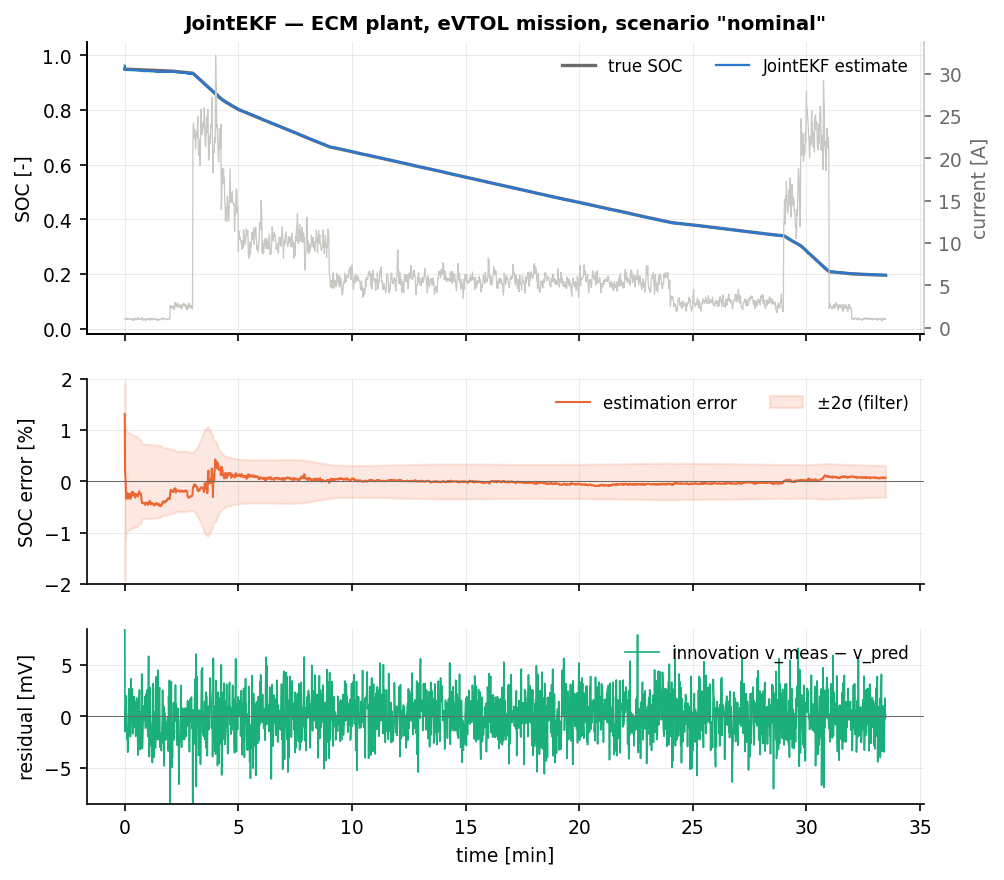
\includegraphics[width=\textwidth]{figures/cell_JointEKF_nominal.png}
\caption{JointEKF on the nominal eVTOL mission: true and estimated SOC (top), estimation error with the $\pm 2\sigma$ band (middle), voltage residual (bottom).}
\end{figure}
\begin{figure}[H]\centering
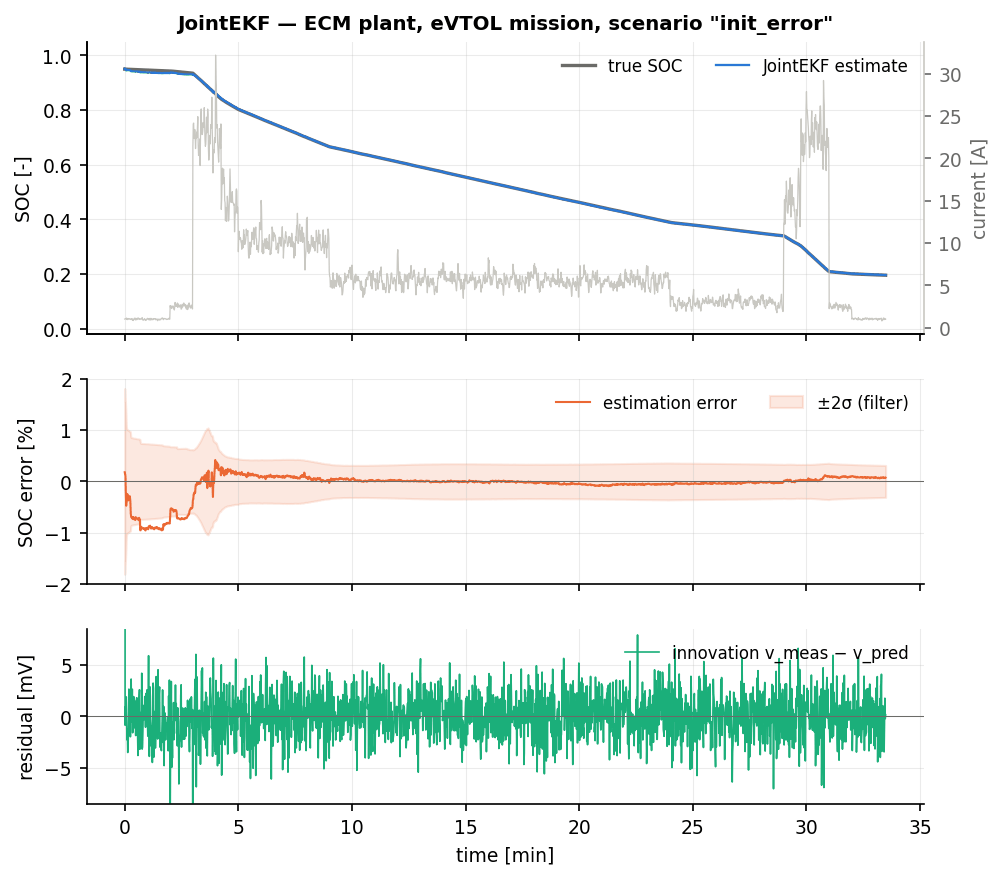
\includegraphics[width=\textwidth]{figures/cell_JointEKF_init_error.png}
\caption{JointEKF with a \SI{35}{\percent} initial SOC error.}
\end{figure}

All figures below are means over three seeds on the eVTOL profile.  On the ECM plant the joint
EKF reaches $\text{RMSE}=0.0011$ and $\text{RMSE}_\text{ss}=0.0005$ on \texttt{nominal} with
immediate convergence, against $0.0015/0.0005$ for the plain EKF and $0.0020/0.0004$ for the UKF
measured in the same run.  On \texttt{init\_error} it converges at $t=\SI{0}{\second}$ with
$\text{RMSE}=0.0028$.  Both acceptance criteria are met and no scenario diverges in any seed.

The decisive result is \texttt{aged\_cell}, the scenario the method exists for.  The truth cell has
lost \SI{15}{\percent} of its capacity ($Q_\text{true}=\SI{4.25}{\ampere\hour}$) and grown its
resistance by \SI{37.5}{\percent}, while the estimator is commissioned with the beginning-of-life
values.  The plain EKF degrades to $\text{RMSE}_\text{ss}=0.0152$; the joint EKF stays at
$0.0005$, a factor of thirty, and ends the flight with
$\texttt{capacity\_err\_end}=\SI{+0.047}{\ampere\hour}$, i.e.\ it recovers about
\SI{4.28}{\ampere\hour} of a true \SI{4.23}{\ampere\hour} --- an error of \SI{0.9}{\percent} of
nameplate after a single \SI{33.5}{\minute} flight.  The residual is of the order of the
\SI{+0.5}{\percent} current-sensor scale-factor error of the nominal sensor model, as predicted by
the identifiability argument of Section~\ref{sec:je-obs}.  The three
capacity figures requested for comparison across the family are
\begin{center}
\begin{tabular}{@{}lrr@{}}
\toprule
Scenario & $Q_\text{true}$ (\si{\ampere\hour}) & \texttt{capacity\_err\_end} (\si{\ampere\hour})\\
\midrule
\texttt{nominal}      & 5.00 & $+0.050$\\
\texttt{aged\_cell}   & 4.25 & $+0.047$\\
\texttt{current\_bias}& 5.00 & $+0.322$\\
\bottomrule
\end{tabular}
\end{center}
The \texttt{current\_bias} row is the textbook illustration of the structural limitation: with a
\SI{+2}{\percent} gain error and a \SI{250}{\milli\ampere} offset the filter reports
\SI{5.31}{\ampere\hour}.  A \SI{2}{\percent} gain error alone accounts for
\SI{0.10}{\ampere\hour}, and the offset integrates to \SI{0.14}{\ampere\hour} over the
\SI{2010}{\second} mission against an SOC swing of $0.75$, i.e.\ a further
\SI{0.19}{\ampere\hour}; the sum is of the order of the observed bias.  The filter is not wrong, the problem is
unidentifiable, exactly as \cite{zhao2017observability,lin2018sensorbias} predict.

Where the joint EKF is \emph{worse} than the plain EKF is equally instructive.  On
\texttt{param\_mismatch} (the estimator is given $R_1$ \SI{30}{\percent} high and $\tau_2$
\SI{50}{\percent} high, neither of which is in $\vtheta$) the SOC error is no better than the plain
EKF's ($\text{RMSE}_\text{ss}=0.0120$ against $0.0136$) and the capacity is biased by
\SI{+0.102}{\ampere\hour}: the filter has absorbed part of a polarisation error into the capacity.
On \texttt{sensor\_dropout} the \SI{15}{\second} stuck-voltage fault at $t=\SI{200}{\second}$ ---
during the take-off hover, when the current is \SI{22}{\ampere} --- produces a sustained
innovation that is integrated straight into the parameter block:
$\text{RMSE}_\text{ss}=0.0142$ against the EKF's $0.0046$, with
$\texttt{capacity\_err\_end}=\SI{+0.404}{\ampere\hour}$.  On \texttt{preisach}, where the truth cell
carries a Preisach loop that the one-state hysteresis model cannot represent, the capacity ends
\SI{+0.231}{\ampere\hour} high.  In every case the mechanism is the same: the augmented
filter has no way to tell ``the model is wrong'' from ``the parameters are wrong'', so every
unmodelled residual is spent on $\vtheta$.  The dual EKF of Chapter~\ref{ch:dualekf} carries an
explicit remedy (an innovation-based floor on the parameter filter's measurement noise); the joint
formulation, having only one covariance, cannot apply it selectively to $\vtheta$.  A robust variant (Huber or Student-$t$ innovation
weighting, Chapter~\ref{ch:huberekf}) would fix the outlier and dropout columns; an innovation gate
applied only to the parameter block was tried and rejected, because on this mission the residual
during the high-current transients is dominated by ECM model error rather than sensor noise, so any
gate tight enough to catch a \SI{50}{\milli\volt} outlier also rejects the most informative
samples.

\paragraph{The electrochemical plant.}  On the SPM plant, where the estimator runs an ECM fitted to
an electrochemical cell and therefore carries a structured few-millivolt voltage model error, the
joint EKF reaches $\text{RMSE}_\text{ss}=0.0211$ on \texttt{nominal} against the plain EKF's
$0.0373$, and beats the plain EKF in all nine SPM scenarios (worst case $0.0506$ against the EKF's
$0.0804$).  Unlike the dual EKF, whose separate parameter covariance needed a dedicated remedy
(Chapter~\ref{ch:dualekf}), the joint filter degrades gracefully by construction: the model error
enters the single shared covariance, which keeps the state and parameter corrections mutually
consistent even when neither is right.  The capacity it reports on that plant
(\SI{+0.10}{\ampere\hour} on \texttt{nominal}) is of limited meaning, since the ``true'' capacity of
a single-particle cell is not the capacity of the ECM fitted to it.

\paragraph{Multi-flight capacity tracking.}  Over a 120-flight accelerated ageing study
(\texttt{bench\_soh --flights 120 --accel 3}), in which the true capacity falls from \SI{5.00}{} to
\SI{3.95}{\ampere\hour}, the joint EKF tracks it with a capacity RMSE of
\SI{26}{\milli\ampere\hour} over flights $11$--$120$ and a final error of
\SI{+21}{\milli\ampere\hour} --- the irreducible \SI{+0.5}{\percent} current-sensor scale-factor
bias --- with a mean per-flight SOC RMSE of $0.0011$, the best of the five SOH methods.

Cost: \SI{1.87}{\micro\second}/step and \SI{4648}{\byte}, against \SI{0.48}{\micro\second} and
\SI{4336}{\byte} for the EKF --- a $3.9\times$ penalty dominated by the model copies in the
numerical parameter Jacobian, not by the $6\times6$ algebra.

\section{Summary}
Use the joint EKF when the cell model's parameters are the dominant error source and the mission
provides enough ampere-hour throughput to make the capacity observable: on the aged cell it turns a
\SI{1.5}{\percent} SOC error into a \SI{0.05}{\percent} one, delivers a capacity estimate good to
\SI{0.9}{\percent} of nameplate within one flight and to \SI{26}{\milli\ampere\hour} over a
120-flight ageing study, for $3.9\times$ the cost of an EKF.  Do not
use it when the current sensor's scale factor is unknown --- capacity and gain are not separately
identifiable and the filter will silently report their product --- nor on data with voltage
outliers or sensor faults, because the augmented filter has no mechanism to distinguish model error
from parameter error and will integrate the fault into $\hat{Q}$.  If either of those risks is
real, prefer the dual EKF of Chapter~\ref{ch:dualekf}, whose parameter filter can be tuned
separately from the state filter, or the dedicated AWTLS capacity estimator of
Chapter~\ref{ch:awtls}, whose anchor-level consistency test rejects the corrupted data outright.
